\documentclass[twoside]{book}

% Packages required by doxygen
\usepackage{calc}
\usepackage{doxygen}
\usepackage{graphicx}
\usepackage[utf8]{inputenc}
\usepackage{makeidx}
\usepackage{multicol}
\usepackage{multirow}
\usepackage{fixltx2e}
\PassOptionsToPackage{warn}{textcomp}
\usepackage{textcomp}
\usepackage[nointegrals]{wasysym}
\usepackage[table]{xcolor}

% Font selection
\usepackage[T1]{fontenc}
\usepackage{mathptmx}
\usepackage[scaled=.90]{helvet}
\usepackage{courier}
\usepackage{amssymb}
\usepackage{sectsty}
\renewcommand{\familydefault}{\sfdefault}
\allsectionsfont{%
  \fontseries{bc}\selectfont%
  \color{darkgray}%
}
\renewcommand{\DoxyLabelFont}{%
  \fontseries{bc}\selectfont%
  \color{darkgray}%
}
\newcommand{\+}{\discretionary{\mbox{\scriptsize$\hookleftarrow$}}{}{}}

% Page & text layout
\usepackage{geometry}
\geometry{%
  a4paper,%
  top=2.5cm,%
  bottom=2.5cm,%
  left=2.5cm,%
  right=2.5cm%
}
\tolerance=750
\hfuzz=15pt
\hbadness=750
\setlength{\emergencystretch}{15pt}
\setlength{\parindent}{0cm}
\setlength{\parskip}{0.2cm}
\makeatletter
\renewcommand{\paragraph}{%
  \@startsection{paragraph}{4}{0ex}{-1.0ex}{1.0ex}{%
    \normalfont\normalsize\bfseries\SS@parafont%
  }%
}
\renewcommand{\subparagraph}{%
  \@startsection{subparagraph}{5}{0ex}{-1.0ex}{1.0ex}{%
    \normalfont\normalsize\bfseries\SS@subparafont%
  }%
}
\makeatother

% Headers & footers
\usepackage{fancyhdr}
\pagestyle{fancyplain}
\fancyhead[LE]{\fancyplain{}{\bfseries\thepage}}
\fancyhead[CE]{\fancyplain{}{}}
\fancyhead[RE]{\fancyplain{}{\bfseries\leftmark}}
\fancyhead[LO]{\fancyplain{}{\bfseries\rightmark}}
\fancyhead[CO]{\fancyplain{}{}}
\fancyhead[RO]{\fancyplain{}{\bfseries\thepage}}
\fancyfoot[LE]{\fancyplain{}{}}
\fancyfoot[CE]{\fancyplain{}{}}
\fancyfoot[RE]{\fancyplain{}{\bfseries\scriptsize Generated on Fri Aug 8 2014 12\+:17\+:18 for Soci\+Plus by Doxygen }}
\fancyfoot[LO]{\fancyplain{}{\bfseries\scriptsize Generated on Fri Aug 8 2014 12\+:17\+:18 for Soci\+Plus by Doxygen }}
\fancyfoot[CO]{\fancyplain{}{}}
\fancyfoot[RO]{\fancyplain{}{}}
\renewcommand{\footrulewidth}{0.4pt}
\renewcommand{\chaptermark}[1]{%
  \markboth{#1}{}%
}
\renewcommand{\sectionmark}[1]{%
  \markright{\thesection\ #1}%
}

% Indices & bibliography
\usepackage{natbib}
\usepackage[titles]{tocloft}
\setcounter{tocdepth}{3}
\setcounter{secnumdepth}{5}
\makeindex

% Hyperlinks (required, but should be loaded last)
\usepackage{ifpdf}
\ifpdf
  \usepackage[pdftex,pagebackref=true]{hyperref}
\else
  \usepackage[ps2pdf,pagebackref=true]{hyperref}
\fi
\hypersetup{%
  colorlinks=true,%
  linkcolor=blue,%
  citecolor=blue,%
  unicode%
}

% Custom commands
\newcommand{\clearemptydoublepage}{%
  \newpage{\pagestyle{empty}\cleardoublepage}%
}


%===== C O N T E N T S =====

\begin{document}

% Titlepage & ToC
\hypersetup{pageanchor=false,
             bookmarks=true,
             bookmarksnumbered=true,
             pdfencoding=unicode
            }
\pagenumbering{roman}
\begin{titlepage}
\vspace*{7cm}
\begin{center}%
{\Large Soci\+Plus }\\
\vspace*{1cm}
{\large Generated by Doxygen 1.8.7}\\
\vspace*{0.5cm}
{\small Fri Aug 8 2014 12:17:18}\\
\end{center}
\end{titlepage}
\clearemptydoublepage
\tableofcontents
\clearemptydoublepage
\pagenumbering{arabic}
\hypersetup{pageanchor=true}

%--- Begin generated contents ---
\chapter{Hierarchical Index}
\section{Class Hierarchy}
This inheritance list is sorted roughly, but not completely, alphabetically\+:\begin{DoxyCompactList}
\item \contentsline{section}{Soci\+Plus\+:\+:Soci\+Plus\+Connection}{\pageref{class_soci_plus_1_1_soci_plus_connection}}{}
\item \contentsline{section}{Soci\+Plus\+:\+:Soci\+Plus\+Model}{\pageref{class_soci_plus_1_1_soci_plus_model}}{}
\begin{DoxyCompactList}
\item \contentsline{section}{Soci\+Plus\+:\+:Soci\+Plus\+Table\+Model}{\pageref{class_soci_plus_1_1_soci_plus_table_model}}{}
\begin{DoxyCompactList}
\item \contentsline{section}{Soci\+Plus\+:\+:Soci\+Plus\+Data\+Table\+Model}{\pageref{class_soci_plus_1_1_soci_plus_data_table_model}}{}
\end{DoxyCompactList}
\end{DoxyCompactList}
\item \contentsline{section}{Soci\+Plus\+:\+:Soci\+Plus\+Model\+Cell}{\pageref{class_soci_plus_1_1_soci_plus_model_cell}}{}
\item \contentsline{section}{Soci\+Plus\+:\+:Soci\+Plus\+Model\+Row}{\pageref{class_soci_plus_1_1_soci_plus_model_row}}{}
\item \contentsline{section}{Soci\+Plus\+:\+:Soci\+Plus\+Query}{\pageref{class_soci_plus_1_1_soci_plus_query}}{}
\end{DoxyCompactList}

\chapter{Class Index}
\section{Class List}
Here are the classes, structs, unions and interfaces with brief descriptions\+:\begin{DoxyCompactList}
\item\contentsline{section}{\hyperlink{class_soci_plus_1_1_soci_plus_connection}{Soci\+Plus\+::\+Soci\+Plus\+Connection} }{\pageref{class_soci_plus_1_1_soci_plus_connection}}{}
\item\contentsline{section}{\hyperlink{class_soci_plus_1_1_soci_plus_data_table_model}{Soci\+Plus\+::\+Soci\+Plus\+Data\+Table\+Model} }{\pageref{class_soci_plus_1_1_soci_plus_data_table_model}}{}
\item\contentsline{section}{\hyperlink{class_soci_plus_1_1_soci_plus_model}{Soci\+Plus\+::\+Soci\+Plus\+Model} }{\pageref{class_soci_plus_1_1_soci_plus_model}}{}
\item\contentsline{section}{\hyperlink{class_soci_plus_1_1_soci_plus_model_cell}{Soci\+Plus\+::\+Soci\+Plus\+Model\+Cell} }{\pageref{class_soci_plus_1_1_soci_plus_model_cell}}{}
\item\contentsline{section}{\hyperlink{class_soci_plus_1_1_soci_plus_model_row}{Soci\+Plus\+::\+Soci\+Plus\+Model\+Row} }{\pageref{class_soci_plus_1_1_soci_plus_model_row}}{}
\item\contentsline{section}{\hyperlink{class_soci_plus_1_1_soci_plus_query}{Soci\+Plus\+::\+Soci\+Plus\+Query} }{\pageref{class_soci_plus_1_1_soci_plus_query}}{}
\item\contentsline{section}{\hyperlink{class_soci_plus_1_1_soci_plus_table_model}{Soci\+Plus\+::\+Soci\+Plus\+Table\+Model} }{\pageref{class_soci_plus_1_1_soci_plus_table_model}}{}
\end{DoxyCompactList}

\chapter{Class Documentation}
\hypertarget{class_soci_plus_1_1_soci_plus_connection}{\section{Soci\+Plus\+:\+:Soci\+Plus\+Connection Class Reference}
\label{class_soci_plus_1_1_soci_plus_connection}\index{Soci\+Plus\+::\+Soci\+Plus\+Connection@{Soci\+Plus\+::\+Soci\+Plus\+Connection}}
}
\subsection*{Public Member Functions}
\begin{DoxyCompactItemize}
\item 
\hypertarget{class_soci_plus_1_1_soci_plus_connection_ae6ddbdb3d9b9c247c76b2e48cf4ae7d7}{{\bfseries Soci\+Plus\+Connection} (string driver, string connection\+String)}\label{class_soci_plus_1_1_soci_plus_connection_ae6ddbdb3d9b9c247c76b2e48cf4ae7d7}

\item 
\hypertarget{class_soci_plus_1_1_soci_plus_connection_a77b4950b22541ccd7d9278389919e51b}{session \& {\bfseries Get\+Session} ()}\label{class_soci_plus_1_1_soci_plus_connection_a77b4950b22541ccd7d9278389919e51b}

\item 
\hypertarget{class_soci_plus_1_1_soci_plus_connection_afeb82c426513a4a735809bdd6ff24daa}{void {\bfseries Open} ()}\label{class_soci_plus_1_1_soci_plus_connection_afeb82c426513a4a735809bdd6ff24daa}

\item 
\hypertarget{class_soci_plus_1_1_soci_plus_connection_a4681c2cd9bbfe6c4502b76b687ab0b27}{void {\bfseries Close} ()}\label{class_soci_plus_1_1_soci_plus_connection_a4681c2cd9bbfe6c4502b76b687ab0b27}

\item 
\hypertarget{class_soci_plus_1_1_soci_plus_connection_ae71f7b2a44a7c23b11217c8d7cabbec9}{void {\bfseries Begin} ()}\label{class_soci_plus_1_1_soci_plus_connection_ae71f7b2a44a7c23b11217c8d7cabbec9}

\item 
\hypertarget{class_soci_plus_1_1_soci_plus_connection_afc0284ab52d9a36939fe239fe35f0e94}{void {\bfseries Commit} ()}\label{class_soci_plus_1_1_soci_plus_connection_afc0284ab52d9a36939fe239fe35f0e94}

\item 
\hypertarget{class_soci_plus_1_1_soci_plus_connection_a364bafdc70ca2bd98d9a726ad4490aa1}{void {\bfseries Rollback} ()}\label{class_soci_plus_1_1_soci_plus_connection_a364bafdc70ca2bd98d9a726ad4490aa1}

\item 
\hypertarget{class_soci_plus_1_1_soci_plus_connection_aa67b916a13243d0d98c96914ff15d91f}{const string \& {\bfseries Get\+Driver} ()}\label{class_soci_plus_1_1_soci_plus_connection_aa67b916a13243d0d98c96914ff15d91f}

\item 
\hypertarget{class_soci_plus_1_1_soci_plus_connection_ab6b4dfadd0f60b8d0d1c25b60cc52779}{const string \& {\bfseries Get\+Connection\+String} ()}\label{class_soci_plus_1_1_soci_plus_connection_ab6b4dfadd0f60b8d0d1c25b60cc52779}

\end{DoxyCompactItemize}
\subsection*{Protected Attributes}
\begin{DoxyCompactItemize}
\item 
\hypertarget{class_soci_plus_1_1_soci_plus_connection_ac7cc98a7a2a789ed882335e23d2b5758}{session $\ast$ {\bfseries m\+\_\+sql}}\label{class_soci_plus_1_1_soci_plus_connection_ac7cc98a7a2a789ed882335e23d2b5758}

\item 
\hypertarget{class_soci_plus_1_1_soci_plus_connection_a7b49011fd8c124f5a0827f33e09c003f}{string {\bfseries m\+\_\+driver}}\label{class_soci_plus_1_1_soci_plus_connection_a7b49011fd8c124f5a0827f33e09c003f}

\item 
\hypertarget{class_soci_plus_1_1_soci_plus_connection_acde14f932cc6cbe0a0302b5da31caa89}{string {\bfseries m\+\_\+connection\+String}}\label{class_soci_plus_1_1_soci_plus_connection_acde14f932cc6cbe0a0302b5da31caa89}

\end{DoxyCompactItemize}


The documentation for this class was generated from the following files\+:\begin{DoxyCompactItemize}
\item 
D\+:/\+Personal/\+Proyectos/sociplus\+\_\+git/trunk/sociplus/include/sociplusconnection.\+h\item 
D\+:/\+Personal/\+Proyectos/sociplus\+\_\+git/trunk/sociplus/src/sociplusconnection.\+cpp\end{DoxyCompactItemize}

\hypertarget{class_soci_plus_1_1_soci_plus_data_table_model}{\section{Soci\+Plus\+:\+:Soci\+Plus\+Data\+Table\+Model Class Reference}
\label{class_soci_plus_1_1_soci_plus_data_table_model}\index{Soci\+Plus\+::\+Soci\+Plus\+Data\+Table\+Model@{Soci\+Plus\+::\+Soci\+Plus\+Data\+Table\+Model}}
}
Inheritance diagram for Soci\+Plus\+:\+:Soci\+Plus\+Data\+Table\+Model\+:\begin{figure}[H]
\begin{center}
\leavevmode
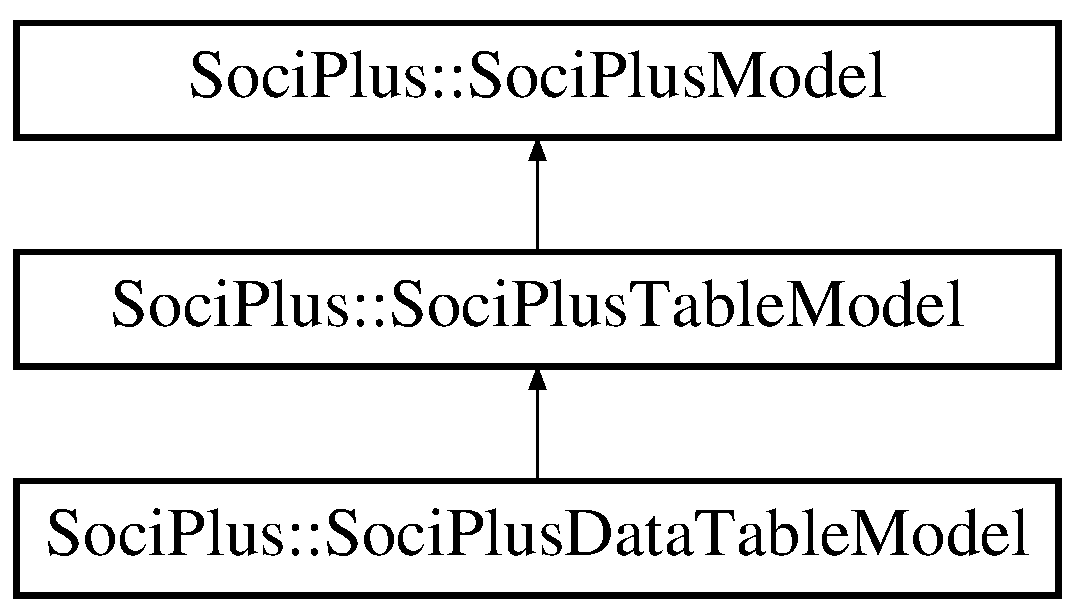
\includegraphics[height=3.000000cm]{class_soci_plus_1_1_soci_plus_data_table_model}
\end{center}
\end{figure}
\subsection*{Public Member Functions}
\begin{DoxyCompactItemize}
\item 
\hypertarget{class_soci_plus_1_1_soci_plus_data_table_model_ae820e6887a04205635aa0fd1b6d68c93}{{\bfseries Soci\+Plus\+Data\+Table\+Model} (int num\+Rows)}\label{class_soci_plus_1_1_soci_plus_data_table_model_ae820e6887a04205635aa0fd1b6d68c93}

\item 
\hypertarget{class_soci_plus_1_1_soci_plus_data_table_model_ad15c45cc7b2b4b224bad7a9bfe36e794}{virtual bool {\bfseries Remove\+Row\+At} (int pos)}\label{class_soci_plus_1_1_soci_plus_data_table_model_ad15c45cc7b2b4b224bad7a9bfe36e794}

\item 
\hypertarget{class_soci_plus_1_1_soci_plus_data_table_model_ab23c2056905cf57489dc5a3cd90d1586}{virtual \hyperlink{class_soci_plus_1_1_soci_plus_model_row}{Soci\+Plus\+Model\+Row} $\ast$ {\bfseries Get\+Row\+At} (int pos)}\label{class_soci_plus_1_1_soci_plus_data_table_model_ab23c2056905cf57489dc5a3cd90d1586}

\item 
\hypertarget{class_soci_plus_1_1_soci_plus_data_table_model_a45314f35c7e804b3bb4c863f00c24b3b}{virtual int {\bfseries Get\+Row\+Count} ()}\label{class_soci_plus_1_1_soci_plus_data_table_model_a45314f35c7e804b3bb4c863f00c24b3b}

\item 
\hypertarget{class_soci_plus_1_1_soci_plus_data_table_model_a77fa62aca7bf84f664a8ce72cd8a890b}{virtual bool {\bfseries Add\+Model} (\hyperlink{class_soci_plus_1_1_soci_plus_model}{Soci\+Plus\+Model} $\ast$model, int row, int col)}\label{class_soci_plus_1_1_soci_plus_data_table_model_a77fa62aca7bf84f664a8ce72cd8a890b}

\item 
\hypertarget{class_soci_plus_1_1_soci_plus_data_table_model_a06ab304eda4dfd6dd7c8aca2fb9a756a}{virtual \hyperlink{class_soci_plus_1_1_soci_plus_model_row}{Soci\+Plus\+Model\+Row} $\ast$ {\bfseries Get\+Header} ()}\label{class_soci_plus_1_1_soci_plus_data_table_model_a06ab304eda4dfd6dd7c8aca2fb9a756a}

\item 
\hypertarget{class_soci_plus_1_1_soci_plus_data_table_model_ac6b814da90881b5b07734c4b3731a951}{virtual \hyperlink{class_soci_plus_1_1_soci_plus_model_row}{Soci\+Plus\+Model\+Row} $\ast$ {\bfseries Get\+Types} ()}\label{class_soci_plus_1_1_soci_plus_data_table_model_ac6b814da90881b5b07734c4b3731a951}

\end{DoxyCompactItemize}
\subsection*{Additional Inherited Members}


The documentation for this class was generated from the following files\+:\begin{DoxyCompactItemize}
\item 
D\+:/\+Personal/\+Proyectos/sociplus\+\_\+git/trunk/sociplus/include/sociplusdatatablemodel.\+h\item 
D\+:/\+Personal/\+Proyectos/sociplus\+\_\+git/trunk/sociplus/src/sociplusdatatablemodel.\+cpp\end{DoxyCompactItemize}

\hypertarget{class_soci_plus_1_1_soci_plus_model}{\section{Soci\+Plus\+:\+:Soci\+Plus\+Model Class Reference}
\label{class_soci_plus_1_1_soci_plus_model}\index{Soci\+Plus\+::\+Soci\+Plus\+Model@{Soci\+Plus\+::\+Soci\+Plus\+Model}}
}
Inheritance diagram for Soci\+Plus\+:\+:Soci\+Plus\+Model\+:\begin{figure}[H]
\begin{center}
\leavevmode
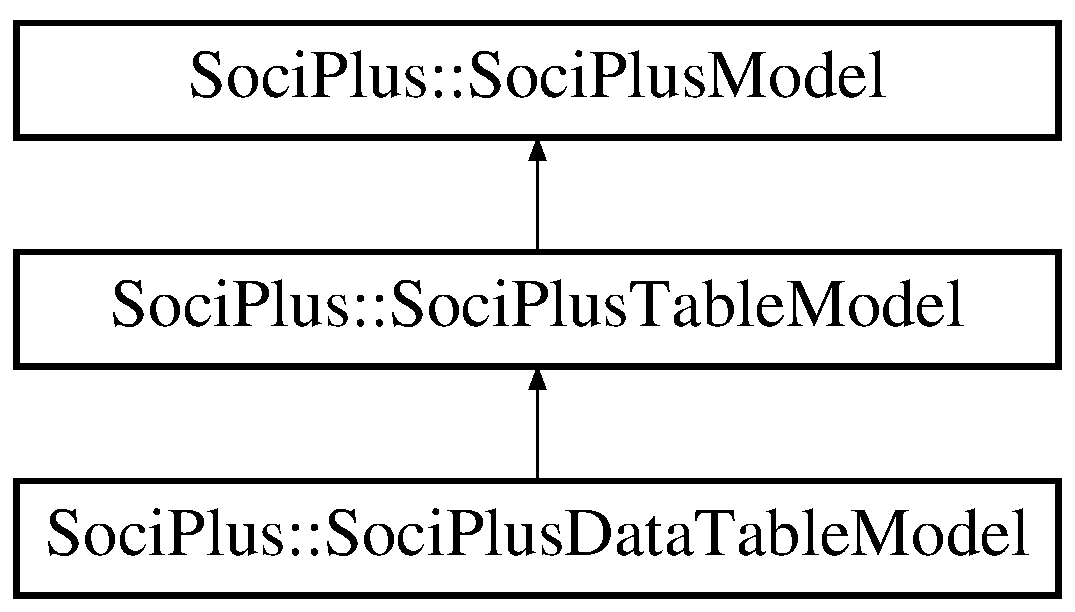
\includegraphics[height=3.000000cm]{class_soci_plus_1_1_soci_plus_model}
\end{center}
\end{figure}
\subsection*{Public Member Functions}
\begin{DoxyCompactItemize}
\item 
\hypertarget{class_soci_plus_1_1_soci_plus_model_aca70ed0e79c366a1b4eceebc88812238}{{\bfseries Soci\+Plus\+Model} (\hyperlink{class_soci_plus_1_1_soci_plus_model_cell}{Soci\+Plus\+Model\+Cell} $\ast$parent=0)}\label{class_soci_plus_1_1_soci_plus_model_aca70ed0e79c366a1b4eceebc88812238}

\item 
\hypertarget{class_soci_plus_1_1_soci_plus_model_abfe63fea6999b82870210fd380a2f186}{virtual \hyperlink{class_soci_plus_1_1_soci_plus_model_row}{Soci\+Plus\+Model\+Row} $\ast$ {\bfseries Add\+Row} ()}\label{class_soci_plus_1_1_soci_plus_model_abfe63fea6999b82870210fd380a2f186}

\item 
\hypertarget{class_soci_plus_1_1_soci_plus_model_a62a53eb94880cf17b44e3b3d4c493249}{virtual bool {\bfseries Add\+Row} (\hyperlink{class_soci_plus_1_1_soci_plus_model_row}{Soci\+Plus\+Model\+Row} $\ast$row)}\label{class_soci_plus_1_1_soci_plus_model_a62a53eb94880cf17b44e3b3d4c493249}

\item 
\hypertarget{class_soci_plus_1_1_soci_plus_model_a96ac7c246892ddf7a5973c477eec0108}{virtual bool {\bfseries Remove\+Row\+At} (int pos)}\label{class_soci_plus_1_1_soci_plus_model_a96ac7c246892ddf7a5973c477eec0108}

\item 
\hypertarget{class_soci_plus_1_1_soci_plus_model_a31340e9ae3b5d00e30d1849856fbc763}{virtual \hyperlink{class_soci_plus_1_1_soci_plus_model_row}{Soci\+Plus\+Model\+Row} $\ast$ {\bfseries Detach\+Row\+At} (int pos)}\label{class_soci_plus_1_1_soci_plus_model_a31340e9ae3b5d00e30d1849856fbc763}

\item 
\hypertarget{class_soci_plus_1_1_soci_plus_model_a56d98da17da9aacca90da2bc076e8f59}{virtual \hyperlink{class_soci_plus_1_1_soci_plus_model_row}{Soci\+Plus\+Model\+Row} $\ast$ {\bfseries Get\+Row\+At} (int pos)}\label{class_soci_plus_1_1_soci_plus_model_a56d98da17da9aacca90da2bc076e8f59}

\item 
\hypertarget{class_soci_plus_1_1_soci_plus_model_aa5fc092c0b75fdd39b8ba2b1d83269da}{virtual int {\bfseries Get\+Row\+Count} ()}\label{class_soci_plus_1_1_soci_plus_model_aa5fc092c0b75fdd39b8ba2b1d83269da}

\item 
\hypertarget{class_soci_plus_1_1_soci_plus_model_a8b3daf440214ee5e7b8e7fd60ed00c9b}{virtual bool {\bfseries Add\+Model} (\hyperlink{class_soci_plus_1_1_soci_plus_model}{Soci\+Plus\+Model} $\ast$model, int row, int col)}\label{class_soci_plus_1_1_soci_plus_model_a8b3daf440214ee5e7b8e7fd60ed00c9b}

\item 
\hypertarget{class_soci_plus_1_1_soci_plus_model_a190ebe098407b746b61d3beb93cd1d15}{virtual int {\bfseries Find\+Row\+Pos} (\hyperlink{class_soci_plus_1_1_soci_plus_model_row}{Soci\+Plus\+Model\+Row} $\ast$row)}\label{class_soci_plus_1_1_soci_plus_model_a190ebe098407b746b61d3beb93cd1d15}

\item 
\hypertarget{class_soci_plus_1_1_soci_plus_model_a06ac8f54c0d7fa946247badb76215874}{virtual bool {\bfseries Move} (\hyperlink{class_soci_plus_1_1_soci_plus_model_cell}{Soci\+Plus\+Model\+Cell} $\ast$cell)}\label{class_soci_plus_1_1_soci_plus_model_a06ac8f54c0d7fa946247badb76215874}

\item 
\hypertarget{class_soci_plus_1_1_soci_plus_model_abeb97098429cf653afb74e8f5f3924b9}{virtual \hyperlink{class_soci_plus_1_1_soci_plus_model_cell}{Soci\+Plus\+Model\+Cell} $\ast$ {\bfseries Get\+Parent} ()}\label{class_soci_plus_1_1_soci_plus_model_abeb97098429cf653afb74e8f5f3924b9}

\item 
\hypertarget{class_soci_plus_1_1_soci_plus_model_a505fa84dafc6b5575b947c0d893c1bfd}{virtual void {\bfseries Set\+Parent} (\hyperlink{class_soci_plus_1_1_soci_plus_model_cell}{Soci\+Plus\+Model\+Cell} $\ast$cell)}\label{class_soci_plus_1_1_soci_plus_model_a505fa84dafc6b5575b947c0d893c1bfd}

\item 
\hypertarget{class_soci_plus_1_1_soci_plus_model_a04ce1b7e64e54aa65a59445bf0a20c6f}{virtual void {\bfseries Clear} ()}\label{class_soci_plus_1_1_soci_plus_model_a04ce1b7e64e54aa65a59445bf0a20c6f}

\end{DoxyCompactItemize}
\subsection*{Protected Attributes}
\begin{DoxyCompactItemize}
\item 
\hypertarget{class_soci_plus_1_1_soci_plus_model_ab91d5dbff92f62f21bbf5ab4ed7eb0f6}{\hyperlink{class_soci_plus_1_1_soci_plus_model_cell}{Soci\+Plus\+Model\+Cell} $\ast$ {\bfseries m\+\_\+parent}}\label{class_soci_plus_1_1_soci_plus_model_ab91d5dbff92f62f21bbf5ab4ed7eb0f6}

\item 
\hypertarget{class_soci_plus_1_1_soci_plus_model_a141b0e669ba1bfcf312ec692d3cd2945}{vector$<$ \hyperlink{class_soci_plus_1_1_soci_plus_model_row}{Soci\+Plus\+Model\+Row} $\ast$ $>$ {\bfseries m\+\_\+rows}}\label{class_soci_plus_1_1_soci_plus_model_a141b0e669ba1bfcf312ec692d3cd2945}

\end{DoxyCompactItemize}


The documentation for this class was generated from the following files\+:\begin{DoxyCompactItemize}
\item 
D\+:/\+Personal/\+Proyectos/sociplus\+\_\+git/trunk/sociplus/include/sociplusmodel.\+h\item 
D\+:/\+Personal/\+Proyectos/sociplus\+\_\+git/trunk/sociplus/src/sociplusmodel.\+cpp\end{DoxyCompactItemize}

\hypertarget{class_soci_plus_1_1_soci_plus_model_cell}{\section{Soci\+Plus\+:\+:Soci\+Plus\+Model\+Cell Class Reference}
\label{class_soci_plus_1_1_soci_plus_model_cell}\index{Soci\+Plus\+::\+Soci\+Plus\+Model\+Cell@{Soci\+Plus\+::\+Soci\+Plus\+Model\+Cell}}
}
\subsection*{Public Member Functions}
\begin{DoxyCompactItemize}
\item 
\hypertarget{class_soci_plus_1_1_soci_plus_model_cell_ab9e251e4d2f63e832c9c5bee400c0c0c}{{\bfseries Soci\+Plus\+Model\+Cell} (\hyperlink{class_soci_plus_1_1_soci_plus_model_row}{Soci\+Plus\+Model\+Row} $\ast$parent)}\label{class_soci_plus_1_1_soci_plus_model_cell_ab9e251e4d2f63e832c9c5bee400c0c0c}

\item 
\hypertarget{class_soci_plus_1_1_soci_plus_model_cell_ae25adc0e4fad7280d119ee6889adeea8}{bool {\bfseries Add\+Model} (\hyperlink{class_soci_plus_1_1_soci_plus_model}{Soci\+Plus\+Model} $\ast$model)}\label{class_soci_plus_1_1_soci_plus_model_cell_ae25adc0e4fad7280d119ee6889adeea8}

\item 
\hypertarget{class_soci_plus_1_1_soci_plus_model_cell_a4633ae0e2129dad5e74569591e190063}{\hyperlink{class_soci_plus_1_1_soci_plus_model}{Soci\+Plus\+Model} $\ast$ {\bfseries Get\+Model\+At} (int pos)}\label{class_soci_plus_1_1_soci_plus_model_cell_a4633ae0e2129dad5e74569591e190063}

\item 
\hypertarget{class_soci_plus_1_1_soci_plus_model_cell_a830aa6986f415dec745430f559958a69}{\hyperlink{class_soci_plus_1_1_soci_plus_model}{Soci\+Plus\+Model} $\ast$ {\bfseries Detach\+Model\+At} (int pos)}\label{class_soci_plus_1_1_soci_plus_model_cell_a830aa6986f415dec745430f559958a69}

\item 
\hypertarget{class_soci_plus_1_1_soci_plus_model_cell_a24737b85906a86a3d0f089123a734eb7}{int {\bfseries Get\+Model\+Count} ()}\label{class_soci_plus_1_1_soci_plus_model_cell_a24737b85906a86a3d0f089123a734eb7}

\item 
\hypertarget{class_soci_plus_1_1_soci_plus_model_cell_abd3344bdae57c006d12d5374e0ca36b7}{void {\bfseries Set\+Data} (string data)}\label{class_soci_plus_1_1_soci_plus_model_cell_abd3344bdae57c006d12d5374e0ca36b7}

\item 
\hypertarget{class_soci_plus_1_1_soci_plus_model_cell_aa347d597231cbbb053187fdf355bcf25}{string {\bfseries Get\+Data} ()}\label{class_soci_plus_1_1_soci_plus_model_cell_aa347d597231cbbb053187fdf355bcf25}

\item 
\hypertarget{class_soci_plus_1_1_soci_plus_model_cell_a6f78dc5746eb5b5a8d551e9536f76c91}{int {\bfseries Find\+Model\+Pos} (\hyperlink{class_soci_plus_1_1_soci_plus_model}{Soci\+Plus\+Model} $\ast$model)}\label{class_soci_plus_1_1_soci_plus_model_cell_a6f78dc5746eb5b5a8d551e9536f76c91}

\item 
\hypertarget{class_soci_plus_1_1_soci_plus_model_cell_a55d2a75a2d633e70188f2e5221aee8f2}{void {\bfseries Clear} ()}\label{class_soci_plus_1_1_soci_plus_model_cell_a55d2a75a2d633e70188f2e5221aee8f2}

\end{DoxyCompactItemize}
\subsection*{Protected Attributes}
\begin{DoxyCompactItemize}
\item 
\hypertarget{class_soci_plus_1_1_soci_plus_model_cell_add456f301caaf058df3cad22c4dd1ebc}{\hyperlink{class_soci_plus_1_1_soci_plus_model_row}{Soci\+Plus\+Model\+Row} $\ast$ {\bfseries m\+\_\+parent}}\label{class_soci_plus_1_1_soci_plus_model_cell_add456f301caaf058df3cad22c4dd1ebc}

\item 
\hypertarget{class_soci_plus_1_1_soci_plus_model_cell_adce43583c83cf5df6912c105985f07f9}{string {\bfseries m\+\_\+data}}\label{class_soci_plus_1_1_soci_plus_model_cell_adce43583c83cf5df6912c105985f07f9}

\item 
\hypertarget{class_soci_plus_1_1_soci_plus_model_cell_a0ad962ec0335c2dc642fec8bce9da997}{vector$<$ \hyperlink{class_soci_plus_1_1_soci_plus_model}{Soci\+Plus\+Model} $\ast$ $>$ {\bfseries m\+\_\+models}}\label{class_soci_plus_1_1_soci_plus_model_cell_a0ad962ec0335c2dc642fec8bce9da997}

\end{DoxyCompactItemize}


The documentation for this class was generated from the following files\+:\begin{DoxyCompactItemize}
\item 
D\+:/\+Personal/\+Proyectos/sociplus\+\_\+git/trunk/sociplus/include/sociplusmodelcell.\+h\item 
D\+:/\+Personal/\+Proyectos/sociplus\+\_\+git/trunk/sociplus/src/sociplusmodelcell.\+cpp\end{DoxyCompactItemize}

\hypertarget{class_soci_plus_1_1_soci_plus_model_row}{\section{Soci\+Plus\+:\+:Soci\+Plus\+Model\+Row Class Reference}
\label{class_soci_plus_1_1_soci_plus_model_row}\index{Soci\+Plus\+::\+Soci\+Plus\+Model\+Row@{Soci\+Plus\+::\+Soci\+Plus\+Model\+Row}}
}
\subsection*{Public Member Functions}
\begin{DoxyCompactItemize}
\item 
\hypertarget{class_soci_plus_1_1_soci_plus_model_row_a881edcf6264ec026738141635511fdfb}{{\bfseries Soci\+Plus\+Model\+Row} (\hyperlink{class_soci_plus_1_1_soci_plus_model}{Soci\+Plus\+Model} $\ast$parent)}\label{class_soci_plus_1_1_soci_plus_model_row_a881edcf6264ec026738141635511fdfb}

\item 
\hypertarget{class_soci_plus_1_1_soci_plus_model_row_a5eb96dbe145ed38d598dee95f74279a5}{bool {\bfseries Add\+Model} (\hyperlink{class_soci_plus_1_1_soci_plus_model}{Soci\+Plus\+Model} $\ast$model, int col)}\label{class_soci_plus_1_1_soci_plus_model_row_a5eb96dbe145ed38d598dee95f74279a5}

\item 
\hypertarget{class_soci_plus_1_1_soci_plus_model_row_a503d6587957265cf7f42d01dc2f3a79d}{\hyperlink{class_soci_plus_1_1_soci_plus_model_cell}{Soci\+Plus\+Model\+Cell} $\ast$ {\bfseries Add\+Cell} ()}\label{class_soci_plus_1_1_soci_plus_model_row_a503d6587957265cf7f42d01dc2f3a79d}

\item 
\hypertarget{class_soci_plus_1_1_soci_plus_model_row_aef34131ea253fe8af5d275108839e807}{\hyperlink{class_soci_plus_1_1_soci_plus_model_cell}{Soci\+Plus\+Model\+Cell} $\ast$ {\bfseries Get\+Cell\+At} (int pos)}\label{class_soci_plus_1_1_soci_plus_model_row_aef34131ea253fe8af5d275108839e807}

\item 
\hypertarget{class_soci_plus_1_1_soci_plus_model_row_ad80ad9e027bc08f9818fdd96b8278f7a}{int {\bfseries Get\+Cell\+Count} ()}\label{class_soci_plus_1_1_soci_plus_model_row_ad80ad9e027bc08f9818fdd96b8278f7a}

\item 
\hypertarget{class_soci_plus_1_1_soci_plus_model_row_aeb7a0bcb93a52a5cd00dc29969ed63ef}{void {\bfseries Set\+Parent} (\hyperlink{class_soci_plus_1_1_soci_plus_model}{Soci\+Plus\+Model} $\ast$parent)}\label{class_soci_plus_1_1_soci_plus_model_row_aeb7a0bcb93a52a5cd00dc29969ed63ef}

\item 
\hypertarget{class_soci_plus_1_1_soci_plus_model_row_ad7756bafacd9fece21af8d3eabf3e61e}{bool {\bfseries Move} (\hyperlink{class_soci_plus_1_1_soci_plus_model}{Soci\+Plus\+Model} $\ast$model)}\label{class_soci_plus_1_1_soci_plus_model_row_ad7756bafacd9fece21af8d3eabf3e61e}

\item 
\hypertarget{class_soci_plus_1_1_soci_plus_model_row_a90cced13fc2a3e768e12a51602cf070b}{void {\bfseries Clear} ()}\label{class_soci_plus_1_1_soci_plus_model_row_a90cced13fc2a3e768e12a51602cf070b}

\end{DoxyCompactItemize}
\subsection*{Protected Attributes}
\begin{DoxyCompactItemize}
\item 
\hypertarget{class_soci_plus_1_1_soci_plus_model_row_a0d105c0cb61aa9269fa697f2091d2d73}{\hyperlink{class_soci_plus_1_1_soci_plus_model}{Soci\+Plus\+Model} $\ast$ {\bfseries m\+\_\+parent}}\label{class_soci_plus_1_1_soci_plus_model_row_a0d105c0cb61aa9269fa697f2091d2d73}

\item 
\hypertarget{class_soci_plus_1_1_soci_plus_model_row_af056d661786def3887b957ff713a2783}{vector$<$ \hyperlink{class_soci_plus_1_1_soci_plus_model_cell}{Soci\+Plus\+Model\+Cell} $\ast$ $>$ {\bfseries m\+\_\+cells}}\label{class_soci_plus_1_1_soci_plus_model_row_af056d661786def3887b957ff713a2783}

\end{DoxyCompactItemize}


The documentation for this class was generated from the following files\+:\begin{DoxyCompactItemize}
\item 
D\+:/\+Personal/\+Proyectos/sociplus\+\_\+git/trunk/sociplus/include/sociplusmodelrow.\+h\item 
D\+:/\+Personal/\+Proyectos/sociplus\+\_\+git/trunk/sociplus/src/sociplusmodelrow.\+cpp\end{DoxyCompactItemize}

\hypertarget{class_soci_plus_1_1_soci_plus_query}{\section{Soci\+Plus\+:\+:Soci\+Plus\+Query Class Reference}
\label{class_soci_plus_1_1_soci_plus_query}\index{Soci\+Plus\+::\+Soci\+Plus\+Query@{Soci\+Plus\+::\+Soci\+Plus\+Query}}
}
\subsection*{Public Member Functions}
\begin{DoxyCompactItemize}
\item 
\hypertarget{class_soci_plus_1_1_soci_plus_query_a5a1db365cfb25a265a02451f7d7451ec}{{\bfseries Soci\+Plus\+Query} (\hyperlink{class_soci_plus_1_1_soci_plus_connection}{Soci\+Plus\+Connection} $\ast$connection)}\label{class_soci_plus_1_1_soci_plus_query_a5a1db365cfb25a265a02451f7d7451ec}

\item 
\hypertarget{class_soci_plus_1_1_soci_plus_query_a5420660fd7b62636c4bc3ce569418768}{virtual \hyperlink{class_soci_plus_1_1_soci_plus_data_table_model}{Soci\+Plus\+Data\+Table\+Model} $\ast$ {\bfseries Execute\+To\+Model} (string query)}\label{class_soci_plus_1_1_soci_plus_query_a5420660fd7b62636c4bc3ce569418768}

\end{DoxyCompactItemize}


The documentation for this class was generated from the following files\+:\begin{DoxyCompactItemize}
\item 
D\+:/\+Personal/\+Proyectos/sociplus\+\_\+git/trunk/sociplus/include/sociplusquery.\+h\item 
D\+:/\+Personal/\+Proyectos/sociplus\+\_\+git/trunk/sociplus/src/sociplusquery.\+cpp\end{DoxyCompactItemize}

\hypertarget{class_soci_plus_1_1_soci_plus_table_model}{\section{Soci\+Plus\+:\+:Soci\+Plus\+Table\+Model Class Reference}
\label{class_soci_plus_1_1_soci_plus_table_model}\index{Soci\+Plus\+::\+Soci\+Plus\+Table\+Model@{Soci\+Plus\+::\+Soci\+Plus\+Table\+Model}}
}
Inheritance diagram for Soci\+Plus\+:\+:Soci\+Plus\+Table\+Model\+:\begin{figure}[H]
\begin{center}
\leavevmode
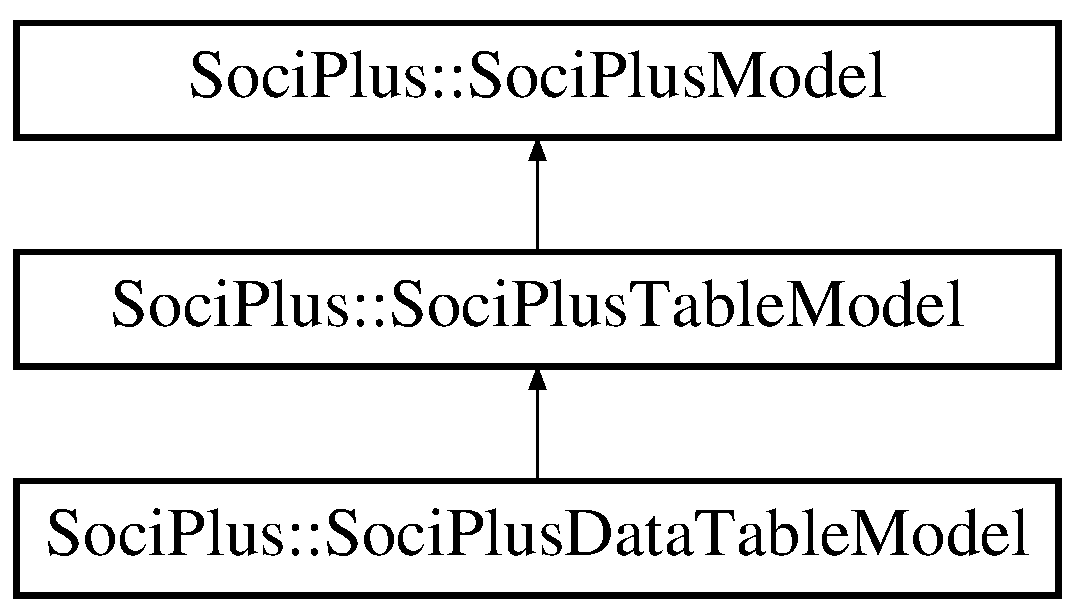
\includegraphics[height=3.000000cm]{class_soci_plus_1_1_soci_plus_table_model}
\end{center}
\end{figure}
\subsection*{Public Member Functions}
\begin{DoxyCompactItemize}
\item 
\hypertarget{class_soci_plus_1_1_soci_plus_table_model_aeb5acf4498ce2936d2ddde7a9258c4d1}{{\bfseries Soci\+Plus\+Table\+Model} (int num\+Cols)}\label{class_soci_plus_1_1_soci_plus_table_model_aeb5acf4498ce2936d2ddde7a9258c4d1}

\item 
\hypertarget{class_soci_plus_1_1_soci_plus_table_model_a184459856f73ae5a7dc670f60287b034}{virtual \hyperlink{class_soci_plus_1_1_soci_plus_model_row}{Soci\+Plus\+Model\+Row} $\ast$ {\bfseries Add\+Row} ()}\label{class_soci_plus_1_1_soci_plus_table_model_a184459856f73ae5a7dc670f60287b034}

\end{DoxyCompactItemize}
\subsection*{Protected Attributes}
\begin{DoxyCompactItemize}
\item 
\hypertarget{class_soci_plus_1_1_soci_plus_table_model_a06ba07e3b3a6e8cbfcf990cbbf754644}{int {\bfseries m\+\_\+num\+Cols}}\label{class_soci_plus_1_1_soci_plus_table_model_a06ba07e3b3a6e8cbfcf990cbbf754644}

\end{DoxyCompactItemize}


The documentation for this class was generated from the following files\+:\begin{DoxyCompactItemize}
\item 
D\+:/\+Personal/\+Proyectos/sociplus\+\_\+git/trunk/sociplus/include/sociplustablemodel.\+h\item 
D\+:/\+Personal/\+Proyectos/sociplus\+\_\+git/trunk/sociplus/src/sociplustablemodel.\+cpp\end{DoxyCompactItemize}

%--- End generated contents ---

% Index
\newpage
\phantomsection
\addcontentsline{toc}{chapter}{Index}
\printindex

\end{document}
